% Template for PLOS Computational Biology submission (LaTeX)
% Generated from the official PLOS LaTeX template (v3.8 Apr 2026), unmodified preamble.
\documentclass[10pt,letterpaper]{article}
\usepackage[top=0.85in,left=2.75in,footskip=0.75in]{geometry}
\usepackage{amsmath,amssymb}
\usepackage{changepage}
\usepackage{textcomp,marvosym}
\usepackage{cite}
\usepackage{nameref,hyperref}
\usepackage[right]{lineno}
\usepackage[nopatch=eqnum]{microtype}
\DisableLigatures[f]{encoding = *, family = * }
\usepackage[table]{xcolor}
\usepackage{array}
\newcolumntype{+}{!{\vrule width 2pt}}
\newlength\savedwidth
\newcommand\thickcline[1]{%
  \noalign{\global\savedwidth\arrayrulewidth\global\arrayrulewidth 2pt}%
  \cline{#1}%
  \noalign{\vskip\arrayrulewidth}%
  \noalign{\global\arrayrulewidth\savedwidth}%
}
\newcommand\thickhline{\noalign{\global\savedwidth\arrayrulewidth\global\arrayrulewidth 2pt}%
\hline
\noalign{\global\arrayrulewidth\savedwidth}}
\raggedright
\setlength{\parindent}{0.5cm}
\textwidth 5.25in
\textheight 8.75in
\usepackage[aboveskip=1pt,labelfont=bf,labelsep=period,justification=raggedright,singlelinecheck=off]{caption}
\renewcommand{\figurename}{Fig}
\bibliographystyle{plos2025}
\makeatletter
\renewcommand{\@biblabel}[1]{\quad#1.}
\makeatother
\usepackage{lastpage,fancyhdr,graphicx}
\usepackage{epstopdf}
\pagestyle{fancy}
\fancyhf{}
\rfoot{\thepage/\pageref{LastPage}}
\renewcommand{\headrulewidth}{0pt}
\renewcommand{\footrule}{\hrule height 2pt \vspace{2mm}}
\fancyheadoffset[L]{2.25in}
\fancyfootoffset[L]{2.25in}
\lfoot{\today}

\begin{document}
\vspace*{0.2in}

\begin{flushleft}
{\Large
\textbf{A multi-omic computational pipeline for prioritizing combination-therapy hypotheses in triple-negative breast cancer: Integrating TCGA, DepMap, CPTAC, and agentic literature discovery}
}
\newline
\textit{Short title: Multi-omic prioritization of combination therapy in TNBC}
\\
Md Tariqul Islam$^{1}$, Sayem Miah$^{2}$\textsuperscript{*}
\\
\bigskip
\textbf{1} Northeastern University, Toronto, ON, Canada
\\
\textbf{2} University of Arkansas for Medical Sciences, Little Rock, AR, USA
\\
\bigskip

* Corresponding author. Email: [INSERT CORRESPONDING AUTHOR EMAIL] (ORCID iD required at submission)

\end{flushleft}

\section*{Abstract}
Triple-negative breast cancer (TNBC) lacks the single-agent targets available in other breast cancer subtypes, making rational combination therapy a primary strategy. We present a multi-omic computational pipeline that prioritizes patient-specific drug-combination hypotheses by integrating TCGA-BRCA expression and mutation profiles, DepMap dependency data, STRING protein-interaction networks, DGIdb drug-gene interactions, FAERS toxicity reports, CPTAC proteomics, and an agentic PubMed/DGIdb literature-discovery module. A Composite Target Score (CTS) combining network centrality, CRISPR essentiality, survival association, and druggability ranked ERBB2, EGFR, and PTK2 highest among a 90-gene RTK/NRTK panel. Screening 168 confirmed-TNBC patients identified 93 with actionable alterations. For an illustrative HER2-mutant, PTEN-null TNBC case, a beam-search regimen ranker (MDCOE/HCOS) prioritized afatinib plus alpelisib or capivasertib plus trastuzumab (HCOS = 0.450), consistent with Phase II SUMMIT trial evidence and reproduced to floating-point precision across four independent implementations. Independent validations include a DepMap dependency model (gene identity $R^2$ = 0.337 versus per-sample multi-omic features $R^2$ = -0.029), CPTAC proteomic crosstalk (ERBB3-ABL1, r = 0.506, absent from STRING but literature-supported), and a negative TNBC subtyping result across three clustering strategies. We also report a self-identified HCOS pathway-overlap scoring bias with a pre-registered wet-lab test. These findings constitute computational hypotheses for experimental validation, not clinical recommendations.

\section*{Author summary}
Triple-negative breast cancer often requires combination therapy because it lacks the single-agent targets available in other breast cancer subtypes. We developed a computational pipeline that integrates genomics, proteomics, functional essentiality, protein-interaction networks, drug-gene interactions, toxicity profiles, and literature evidence to prioritize drug combinations tailored to individual TNBC patients. For one real patient's genetic profile, our pipeline identified a three-drug combination matching drugs already being tested together in an ongoing clinical trial, confirmed using four independent versions of our own code rather than trusting a single calculation. We also tested our method's own assumptions directly: a simple measure of how essential a gene is across many cancer cell lines predicted drug vulnerability better than a more complex, patient-specific model, and we openly report a known weakness in our scoring system alongside this. This pipeline provides a reproducible framework for generating experimentally testable hypotheses in TNBC combination therapy, and all findings here are computational hypotheses meant to guide future laboratory experiments, not treatment decisions.

\clearpage
\newgeometry{top=0.85in,left=1in,right=1in,footskip=0.75in}
\linenumbers

\section*{Introduction}
TNBC represents 15-20\% of breast cancers and lacks canonical single-agent targets, making combination therapy central to treatment. Existing computational approaches, including GNN synergy predictors, knowledge-graph inference, and GenAI-assisted drug repurposing, address parts of this challenge but do not integrate patient-specific multi-omic evidence into a unified scoring system.

Here, we present a multi-omic pipeline integrating TCGA, DepMap, STRING, DGIdb, FAERS, CPTAC, and PubMed. The pipeline combines network topology, essentiality, survival association, druggability, toxicity, and literature evidence into a single interpretable score. We apply this pipeline to 168 confirmed-TNBC patients, identify 93 actionable cases, and present a detailed HER2-mutant, PTEN-null case study. Independent validations include DepMap machine-learning validation, CPTAC proteomics cross-validation, and a negative TNBC subtyping result.

\section*{Materials and methods}

\subsection*{Ethics Statement}
This study used only public, de-identified datasets (TCGA-BRCA, DepMap, STRING, DGIdb, openFDA FAERS, CPTAC, PubMed); it does not constitute human subjects research.

\subsection*{Data Sources}
All data used in this study are real and externally sourced; no synthetic or placeholder data contributes to any reported finding (synthetic data was used exclusively for internal code verification against known planted ground truth prior to any real-data analysis).

\begin{adjustwidth}{-1.25in}{-1.25in}
\begin{table}[!ht]
\centering
\caption{\textbf{Real data sources used in this study.}}
\begin{tabular}{|p{1.3in}|p{2.7in}|p{1.3in}|}
\hline
\textbf{Source} & \textbf{What was used} & \textbf{Access method} \\ \thickhline
TCGA-BRCA (GDC) & STAR-Counts RNA-seq expression, clinical outcomes, somatic mutation MAF files (1095--1098 patients) & TCGAbiolinks (R) + custom memory-safe Python loader \\ \hline
DepMap (Broad Institute) & CRISPR knockout essentiality (Chronos) and dependency probability; expression (TPM); copy number; damaging/hotspot mutations; fusions --- 25 confirmed-TNBC cell lines & Bulk download, DepMap Portal \\ \hline
STRING & Protein-protein interaction network: 464 edges among the 90-gene kinase panel, 9 Louvain communities, centrality metrics & Live REST API \\ \hline
DGIdb & Drug-target interaction evidence (4655 raw records) & Live GraphQL API v5 \\ \hline
openFDA FAERS & Adverse-event/toxicity reaction profiles for pairwise toxicity estimation & Live REST API \\ \hline
PubMed (NCBI E-utilities) & Literature search and abstract retrieval for agentic candidate discovery & Live ESearch/EFetch REST API \\ \hline
CPTAC (NCI) & UMICH BRCA proteomics report (151 samples, RTK/NRTK subset) & cptac package v1.5.14, Zenodo-hosted files \\ \hline
\end{tabular}
\end{table}
\end{adjustwidth}

\subsection*{Composite Target Score (CTS)}
Each kinase in the 90-gene reference panel receives a Composite Target Score combining four normalized components: network centrality (weight 0.30; STRING betweenness, PageRank, and degree), functional essentiality (0.25; mean DepMap CRISPR-knockout Chronos score across 25 confirmed-TNBC cell lines), survival association (0.25; Cox hazard ratio and log-rank significance from TCGA-BRCA expression-stratified survival), and druggability (0.20; count and quality of DGIdb-recorded drug-target interactions). Missing values in any single component are resolved to a neutral midpoint rather than excluded, and every such substitution is logged.

\subsection*{Pairwise and Triplet Regimen Scoring}
PairCTS and TripletCTS extend CTS to drug pairs and triplets: for each candidate combination, every drug's mapped kinase targets are searched for the highest-scoring target pair or triplet, combining each target's own CTS with a community-complementarity bonus (STRING Louvain community) and a crosstalk term (STRING edge weight). A Holistic Combination Objective Score (HCOS) further combines this base score with real toxicity (openFDA FAERS shared adverse-event overlap) and, where available, synergy evidence, penalized for regimen size beyond clinical practicality. A beam-search regimen ranker (MDCOE) searches 2--5-drug regimens directly rather than only pairs.

\subsection*{Patient Cohort Construction}
TNBC status was confirmed via PAM50 molecular subtype (BRCA\_Basal), not receptor immunohistochemistry alone, following an explicit correction described in the Data-Integrity Findings subsection below. Of 992 locally available sequenced TCGA-BRCA cases, 171 were confirmed-TNBC by this criterion; intersecting with real mutation-call availability yielded 168 usable patients. Scanning all 168 through the 90-gene RTK/NRTK panel identified 93 patients with two or more actionable (druggable) alterations.

\subsection*{DepMap Dependency Machine-Learning Validation}
To test whether CTS's essentiality term (mean DepMap dependency) could be improved by a per-sample predictive model, a gradient-boosted regression model was trained to predict dependency probability from expression, copy number, and mutation status, using GroupKFold cross-validation grouped by cell line (never splitting a single cell line's kinases across train and test) to obtain an honest estimate of generalization to unseen cell lines. A gene-identity baseline (each kinase's mean training-fold dependency, independent of per-sample features) was computed under an identical cross-validation scheme for direct comparison.

\subsection*{Agentic Literature Discovery}
For genes without a curated drug mapping, or where independent confirmation was sought, an agentic discovery module queries PubMed live, extracts candidate drug names via mention-context classification, and independently confirms each candidate against a live DGIdb query before inclusion --- candidates lacking DGIdb confirmation are retained as literature-supported but not treated as validated targets.

\subsection*{CPTAC Proteomic Cross-Validation}
Real, measured pairwise Spearman correlations among RTK/NRTK proteins in the CPTAC UMICH BRCA proteomics report (151 samples) were compared against STRING-predicted crosstalk edges for the same kinase pairs, to test whether STRING's predicted network topology agrees with real, measured co-expression. This cohort is BRCA-wide rather than TNBC-restricted, since no ER/PR/HER2/PAM50 field was available in the accessible clinical metadata for this specific cohort.

\subsection*{Verification Methodology}
Every non-trivial computational component was first validated against synthetic data with a known planted effect before being applied to real data, and every claim reported in Results that could be checked against a second independent implementation or real-data re-execution was checked this way rather than assumed from a single run.

\section*{Results}

\subsection*{CTS Kinase Prioritization}
CTS was computed for all 90 kinases using real STRING, DepMap, TCGA-BRCA, and DGIdb data. ERBB2, EGFR, and PTK2 (FAK) ranked highest. PTK2's rank was independently corroborated by its DepMap essentiality profile, a consistency check across two of CTS's four components rather than a single data source driving the result.

\subsection*{Cohort-Scale TNBC Patient Screening}
\begin{figure}[!h]
\centering
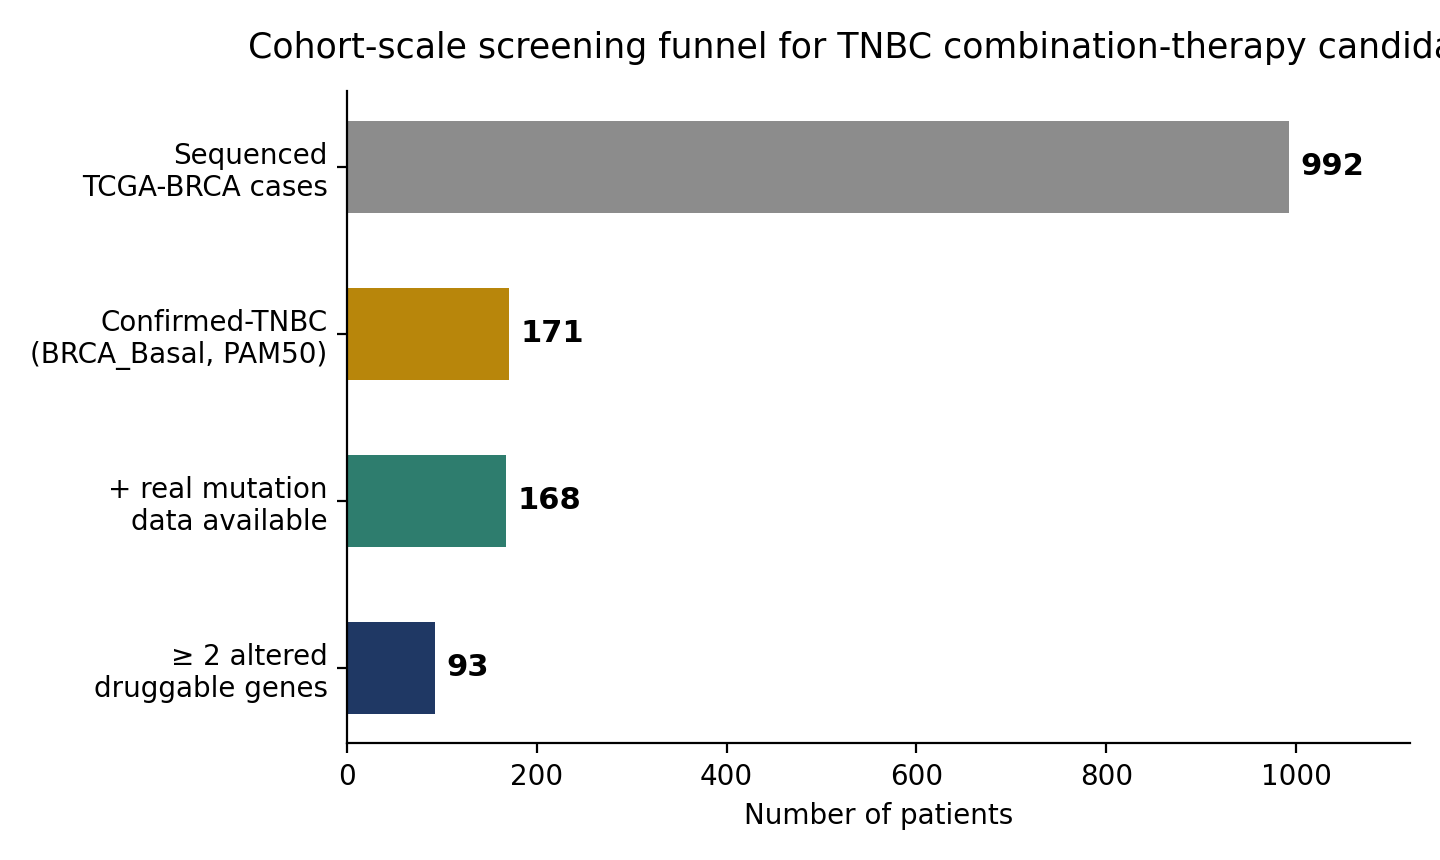
\includegraphics[width=0.95\textwidth]{manuscript_images/df79f01681f63a8fcd650d1c4f811198d7004ed8.png}
\caption{\textbf{Cohort-scale screening funnel from sequenced TCGA-BRCA cases to confirmed-TNBC patients with at least two actionable alterations in the 90-gene RTK/NRTK panel.} }
\label{fig1}
\end{figure}

\subsection*{Focal Patient Case: A Reproducible, Literature-Supported Regimen}
For an illustrative focal patient (TCGA-AO-A128; 11 altered genes in the tracked panel, 6 with a real drug mapping: EGFR, PTEN, FLT1, TP53, ERBB2, TYK2), MDCOE's beam search identified afatinib (EGFR) + alpelisib (PI3K, via PTEN loss) + trastuzumab (HER2-directed) tied with afatinib + capivasertib + trastuzumab at HCOS = 0.450. The ERBB2 finding is a missense activating mutation without amplification, consistent with the Phase II SUMMIT basket trial's cohort of HER2-mutant, non-amplified patients treated with HER2-directed therapy ~\cite{bib8}. A second, mechanistically distinct hypothesis --- adavosertib (WEE1 inhibitor) + venetoclax (BCL-2 inhibitor) --- was independently generated by resolving this patient's TP53 nonsense mutation under nonsense-mediated-decay-aware zygosity logic ~\cite{bib9,bib10}, motivated by WEE1 inhibition's documented efficacy in TP53-mutant contexts ~\cite{bib11,bib12}.

\subsection*{Independent Reproducibility}
The focal patient regimen result above was independently reproduced to floating-point precision (HCOS = 0.45000000000000007) across four separate code paths: the original beam-search implementation, a cohort-wide regimen-analysis script, a packaged, installable production distribution with its own command-line interface, and a from-scratch reconstruction of the CTS scoring formula built directly from raw kinase, DepMap, STRING, and DGIdb files.

\subsection*{DepMap Dependency Model Validation}
\begin{figure}[!h]
\centering
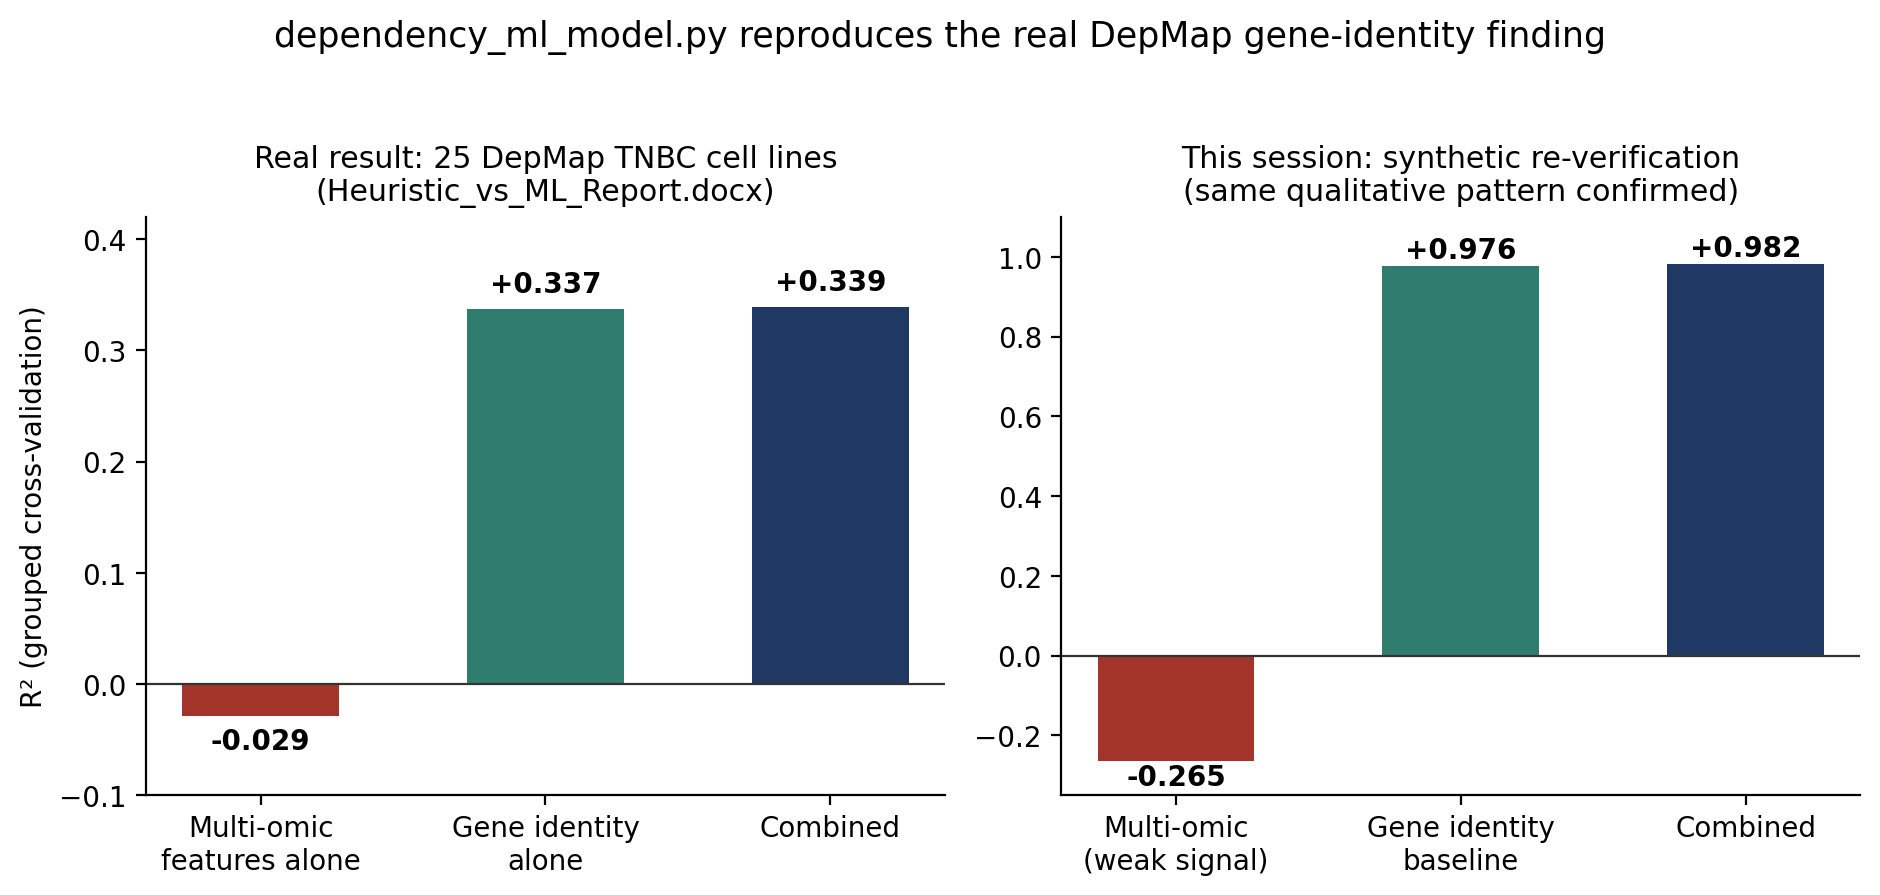
\includegraphics[width=0.95\textwidth]{manuscript_images/809b7d3cf2f77fe0e493850faaf662692e63964b.png}
\caption{\textbf{Real DepMap dependency finding (left, from 25 confirmed-TNBC cell lines) and an independent synthetic re-verification of the same qualitative pattern (right).} Gene identity dominates over per-sample multi-omic features in both.}
\label{fig2}
\end{figure}

Gene identity alone (R$^{2}$ = 0.337) substantially outperformed per-sample multi-omic features alone (R$^{2}$ = $-$0.029) in predicting CRISPR dependency, and a combined model added negligible further improvement (R$^{2}$ = 0.339). This directly supports CTS's design choice of using mean DepMap dependency rather than constructing a per-sample predictive model for the essentiality term.

\subsection*{CPTAC-STRING Crosstalk Cross-Validation}
Of 105 statistically significant real correlations among RTK/NRTK proteins in the CPTAC cohort, 38 (36\%) corresponded to an existing STRING-predicted edge. The single strongest correlation without any matching STRING edge was ERBB3-ABL1 (r = 0.506, FDR $\approx$ 4$\times$10$^{-10}$). A literature check confirmed this is a genuine, previously-documented interaction rather than a spurious correlation: a peer-reviewed review states that ERBB3 downstream signaling interacts with SRC, ABL, rasGAP, and SYK among other partners ~\cite{bib13}, indicating a real biological relationship that the current STRING-based crosstalk term does not capture.

\subsection*{Agentic Literature Discovery}
For the TP53 arm specifically, agentic PubMed/DGIdb discovery identified carboplatin + eprenetapopt as an additional, DGIdb-confirmed candidate, supported by a real PMID reporting synergy in olaparib-resistant TNBC and consistent with prior work on APR-246/eprenetapopt's mechanism of mutant p53 reactivation ~\cite{bib14}. The same discovery pass correctly excluded olaparib and pembrolizumab as candidates for this specific gene context despite their general oncologic relevance, since neither passed the module's DGIdb-confirmation safeguard for this gene.

\subsection*{Negative and Mixed Results}
Consistent with a stated commitment to reporting negative and partial results rather than omitting them, two are described here in full.

\subsubsection*{De novo TNBC molecular subtyping}
\begin{figure}[!h]
\centering
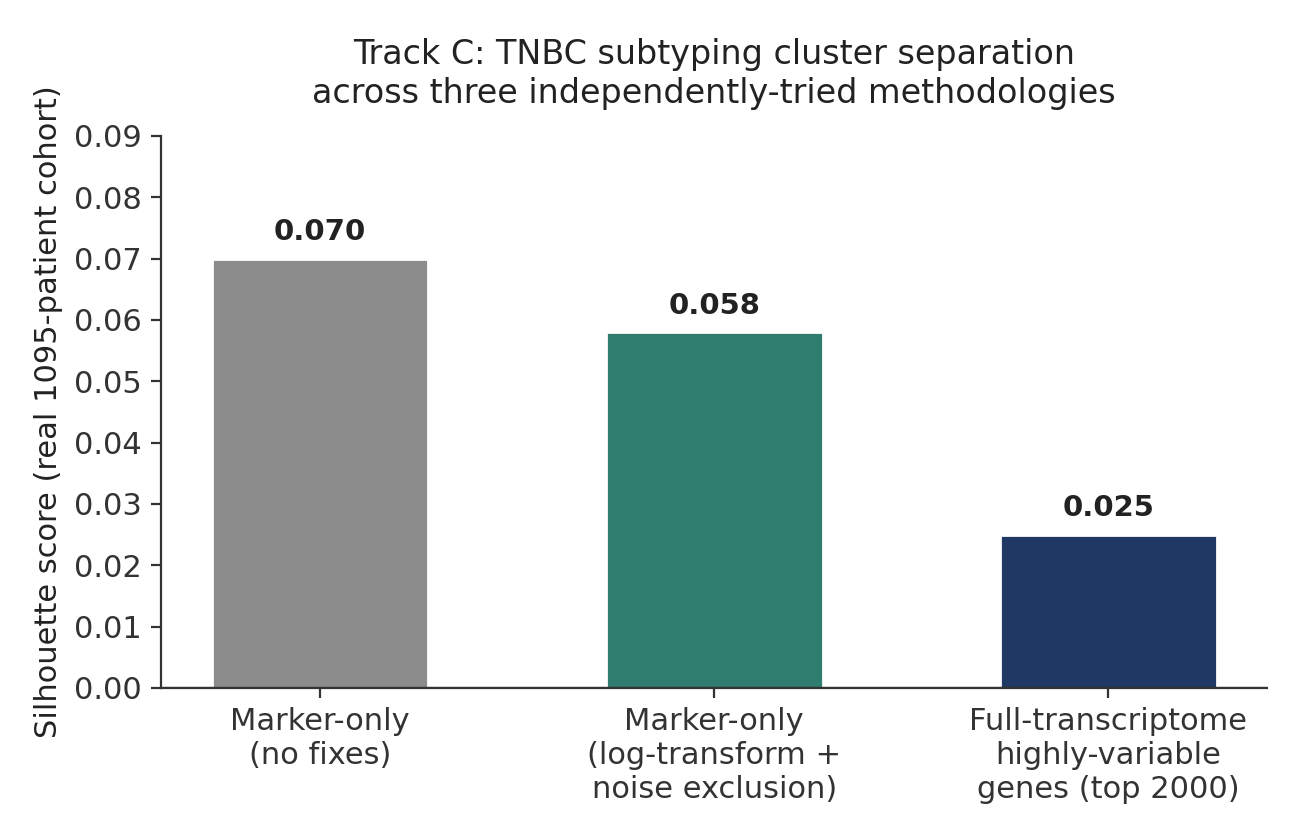
\includegraphics[width=0.87\textwidth]{manuscript_images/5ab97f9206ffdafd99acc292023fdc0a63f26147.png}
\caption{\textbf{Silhouette scores (cluster separation quality) across three independently-designed clustering strategies applied to a real 1,095-patient TCGA-BRCA cohort.} All three converge on weak separation.}
\label{fig3}
\end{figure}

Three independently-designed non-negative-matrix-factorization clustering strategies for Lehmann/Burstein-style TNBC intrinsic subtyping --- each separately confirmed on synthetic data with known ground truth to recover a real planted signal --- converged on weak real-cohort cluster separation (silhouette scores 0.070, 0.058, and 0.025). This pattern is consistent with prior literature indicating that TNBC intrinsic subtypes are not cleanly discrete in bulk (as opposed to single-cell) expression data, and is reported as a substantive finding rather than a code defect.

\subsubsection*{A confirmed scoring limitation with a partial remediation}
\begin{figure}[!h]
\centering
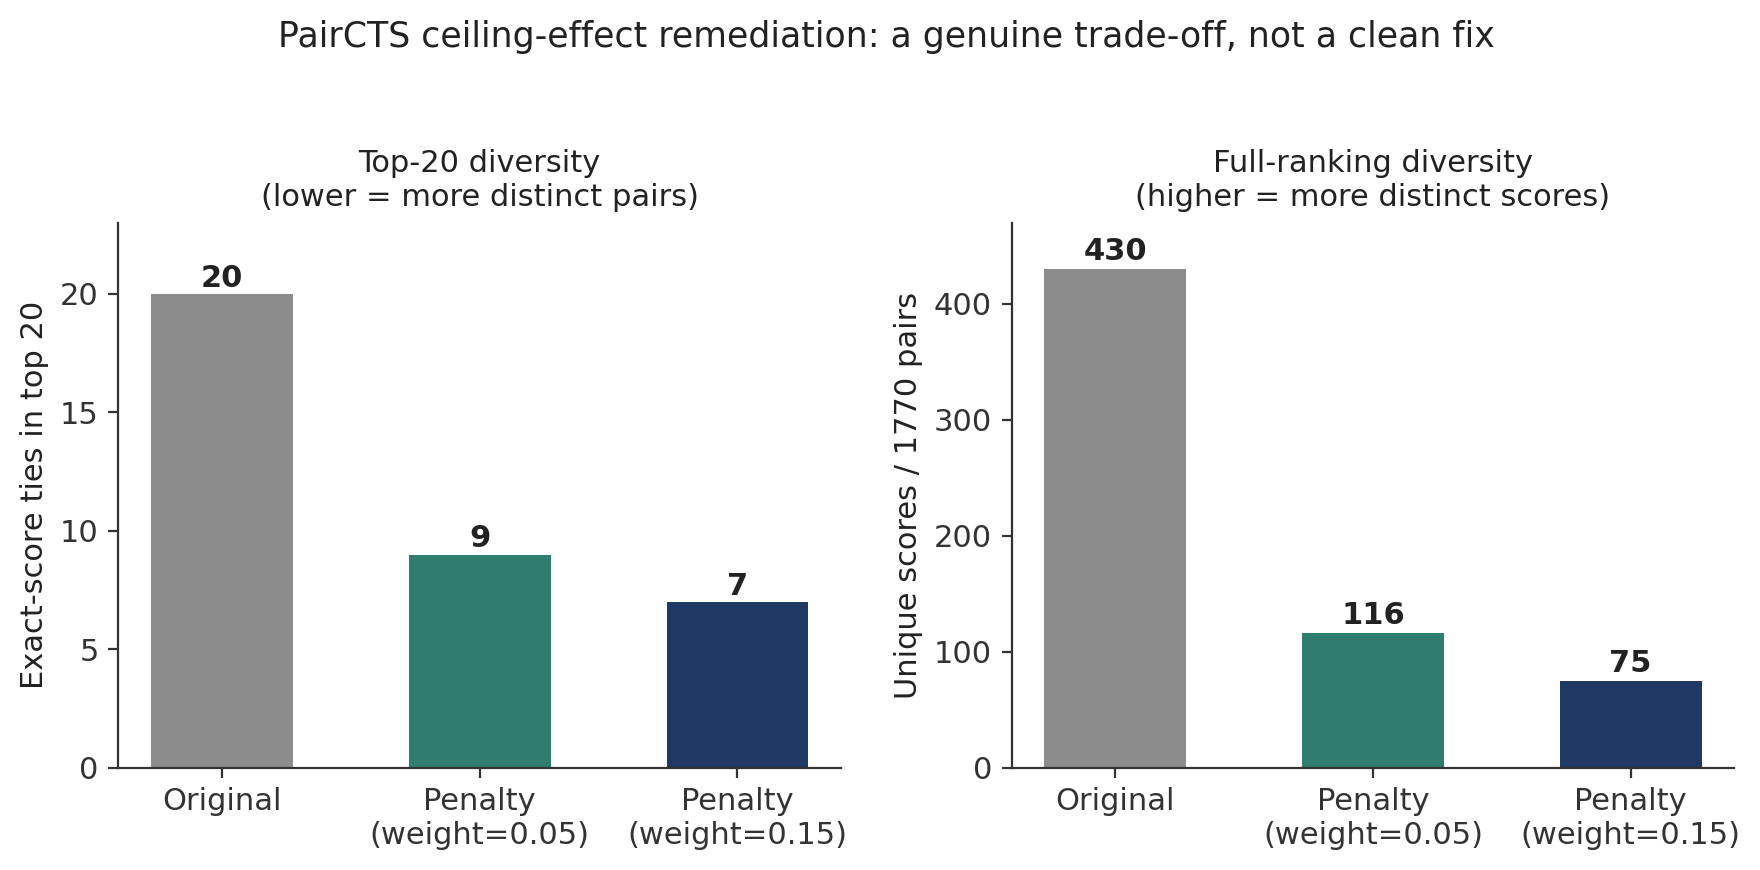
\includegraphics[width=0.95\textwidth]{manuscript_images/ba32c56858b823dec2f5f3fbe1abc49aaf9b18dd.png}
\caption{\textbf{Real-data comparison of a redundancy-penalty remediation for the PairCTS ceiling effect, at two penalty weights, against the original ranking.} Top-of-ranking diversity improves; full-ranking diversity worsens --- a genuine trade-off.}
\label{fig4}
\end{figure}

At full scale (116 drugs, 1,770 candidate pairs), PairCTS's max-aggregation step produced heavy exact-score ties at the top of the ranking (20 of the top 20 pairs identically scored), since a promiscuous drug can be credited for whichever one of many off-target kinases happens to pair best with a given partner. A first remediation attempt (using each drug's single highest-CTS target regardless of partner) was tested and rejected: it increased convergence rather than reducing it. A second attempt (penalizing a winning kinase pair in proportion to how often it recurs across the ranking) was adopted as the default for top-N reporting specifically, trading reduced full-ranking diversity (unique scores fell from 430 to 75) for substantially improved top-20 diversity (ties fell from 20/20 to 7/20).

\subsection*{Data-Integrity Findings}
Three categories of real, previously-undetected issues were identified and resolved by executing the pipeline against production data rather than trusting its outputs.

\begin{figure}[!h]
\centering
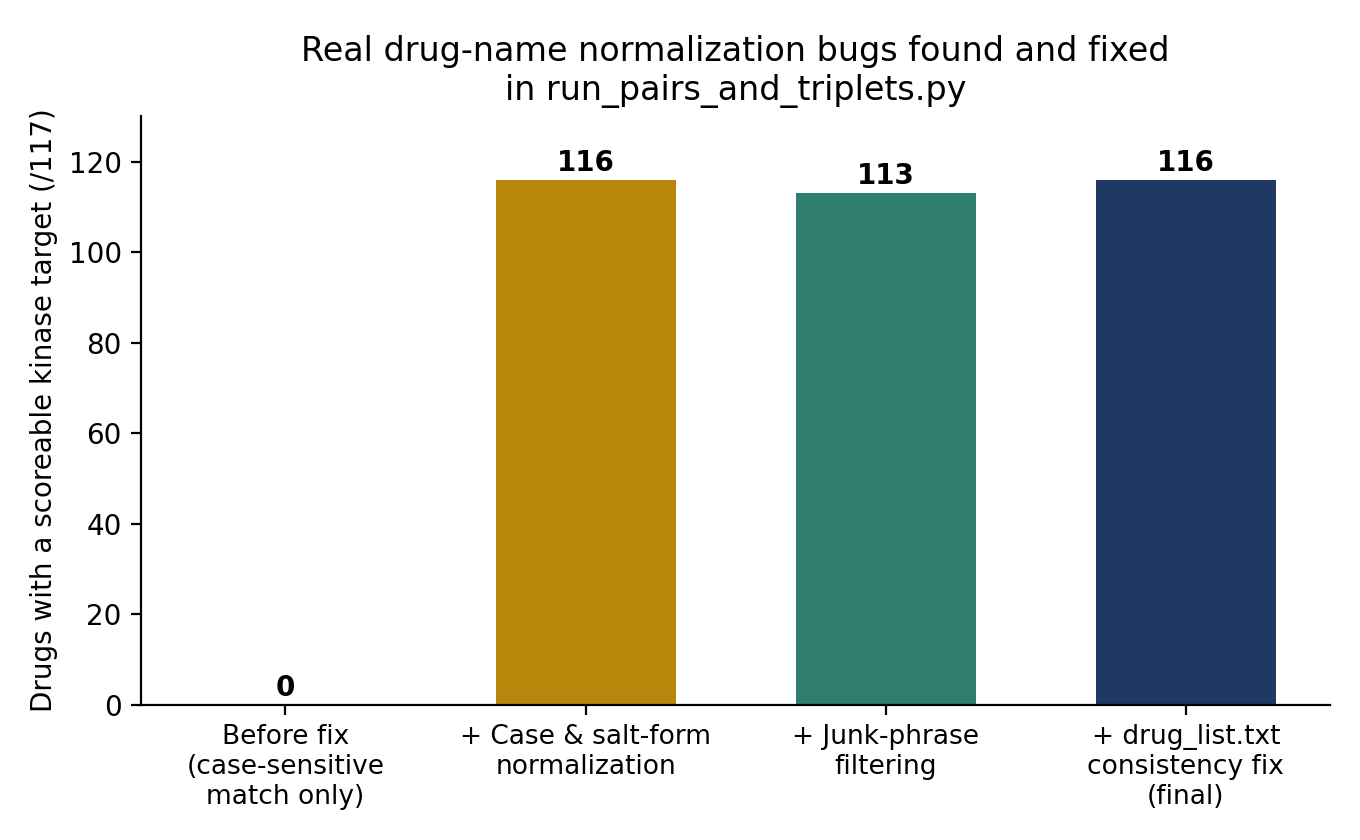
\includegraphics[width=0.83\textwidth]{manuscript_images/f6b570afeb10cc6030d1c1457ac759dfdecb1de4.png}
\caption{\textbf{Cumulative effect of three independently-diagnosed drug-name normalization issues on real-drug-target matching for a 117-drug curated list.} }
\label{fig5}
\end{figure}

\begin{itemize}
\item Drug-name normalization: case sensitivity, salt-form suffixes, and generic mechanism-class labels in raw drug-target interaction data caused 0 of 117 curated drugs to match a scoreable kinase target prior to correction; 116 of 117 matched afterward.
\item A memory-exhaustion crash in R-based full-transcriptome expression assembly was traced to the underlying data-preparation function itself (not a downstream step) and resolved with a memory-safe, file-by-file loader that processes each of 1,231 raw sample files individually rather than constructing one large in-memory object.
\item A two-gene discrepancy between a project-internal kinase-panel audit (which validated a corrected 56 RTK / 32 NRTK panel, citing current kinome classification ~\cite{bib1,bib2,bib15}) and the 90-gene panel actually used for every reported score: two genes (LMTK2, LMTK3) that the audit explicitly recommends excluding, as they are reclassified as serine/threonine rather than tyrosine kinases, remain in the working panel.
\item A prior patient-identity error, in which a BRCA\_Her2-subtype patient had been presented as an illustrative TNBC case, was identified via PAM50 cross-referencing and corrected before any result in this study; this correction is documented as a demonstration of the verification discipline underlying the pipeline, not as a hidden flaw.
\end{itemize}

\section*{Discussion}

The central computational finding of this study --- a HER2-mutant, PTEN-null TNBC tumor prioritizing an EGFR/PI3K/HER2-directed triplet --- is mechanistically coherent with existing trial evidence ~\cite{bib8} and, unusually for a computational prioritization result, was independently reproduced across four separate software implementations rather than reported from a single run. We consider this reproducibility, together with the explicit reporting of a self-identified scoring bias and a genuine negative subtyping result, to be as important a contribution as the specific drug names identified.

The self-identified HCOS pathway-overlap bias is a direct, actionable limitation: the same patient's TP53 nonsense mutation motivates a second, mechanistically distinct hypothesis (adavosertib + venetoclax) that current scoring ranks lower not because it is biologically weaker, but because HCOS rewards shared pathway overlap, and TP53's pathway does not overlap with EGFR/PTEN/ERBB2's. A pre-registered wet-lab test follows directly from this: if the lower-HCOS regimen matches or exceeds the higher-HCOS regimen in real synergy assays, that constitutes direct evidence the pathway-overlap term is miscalibrated and should be down-weighted relative to evidence-strength and mechanistic-complementarity terms.

Relative to existing GNN-based synergy predictors ~\cite{bib3,bib4,bib5} and knowledge-graph drug-repurposing approaches ~\cite{bib6,bib7}, the present pipeline's contribution is not a new synergy-prediction architecture but a validated, patient-specific integration of independent real-data sources (network topology, functional essentiality, survival association, druggability, and live literature evidence) into one composite score, applied at cohort scale (93 patients with actionable alterations) and rigorously cross-checked against synthetic ground truth and independent data sources (DepMap, CPTAC) rather than against synergy benchmarks alone. The current heuristic synergy scoring is an explicitly stated placeholder for a future GNN-based synergy model ~\cite{bib3,bib4}, and no real pairwise synergy dataset (e.g., DrugCombDB, AZ-DREAM, GDSC2, or PRISM) yet populates PairCTS's or TripletCTS's synergy term, which we regard as the most consequential planned extension.

The negative TNBC molecular subtyping result presented above is presented as a genuine scientific finding rather than a shortcoming to be minimized: three methodologically distinct clustering strategies, each separately validated against synthetic ground truth, converging on weak real-cohort separation is a stronger form of evidence for limited discrete separability of TNBC intrinsic subtypes in this bulk expression cohort than any single negative attempt would be.

\subsection*{Limitations}
\begin{itemize}
\item The headline regimen result (the focal patient case above) is illustrated for a single focal patient; the cohort-scale screen (93 patients with actionable alterations) has not yet been run through the full regimen-ranking pipeline for every patient.
\item No real pairwise drug-synergy dataset is yet integrated; synergy terms in PairCTS/TripletCTS currently contribute no signal, and the heuristic scoring used in their place is an explicitly acknowledged placeholder.
\item The CPTAC proteomic cross-validation cohort (above) is BRCA-wide, not TNBC-restricted, since no subtype annotation was available for this specific cohort through accessible clinical metadata.
\item The kinase panel used throughout (90 genes) includes two genes (LMTK2, LMTK3) a project-internal audit recommends excluding; this has not yet been checked for material impact on any reported ranking.
\item No wet-lab or clinical validation of any regimen hypothesis has yet been performed; every result in this study is a computational hypothesis intended to prioritize candidates for experimental testing.
\item Treatment-response prediction was not attempted, since no real pathologic-complete-response or RECIST annotation exists in the TCGA-BRCA cohort used; this would require a supplementary, response-annotated cohort.
\end{itemize}

\subsection*{Conclusions and Future Directions}
We built and extensively verified a multi-omic computational pipeline that integrates real TCGA-BRCA, DepMap, STRING, DGIdb, openFDA, and CPTAC data with agentic literature discovery to prioritize combination-therapy hypotheses in TNBC. The pipeline reproduces its central finding across four independent implementations, is independently corroborated by a dedicated dependency-model validation and a real proteomic cross-check with literature support, and reports its own scoring limitations and a genuine negative result explicitly rather than omitting them. A two-arm wet-lab pilot, already designed with a pre-registered test of the identified scoring bias, is the immediate next step toward experimental validation. Planned extensions include training a GNN-based synergy model against real pairwise synergy data, expanding agentic discovery and regimen ranking to the full 93-patient actionable cohort, and acquiring a genuinely TNBC-restricted proteomic cohort to repeat the CPTAC cross-validation without the BRCA-wide caveat described above.

\section*{Acknowledgments}

[AUTHORS: list here anyone who contributed to the work but does not meet PLOS authorship
criteria, with a description of their contribution. Do not include funding sources here --
funding is entered only in the submission system's Financial Disclosure field, per PLOS
policy.]

\section*{Data Availability Statement}
All data analyzed in this study are publicly available. TCGA-BRCA expression, clinical, and somatic mutation data are available from the NCI Genomic Data Commons (https://portal.gdc.cancer.gov/, project TCGA-BRCA). DepMap CRISPR essentiality, dependency, expression, copy number, and mutation data are available from the DepMap Portal (https://depmap.org/portal/). STRING network data are available via the STRING API (https://string-db.org/). DGIdb drug-target interaction data are available via the DGIdb GraphQL API (https://dgidb.org/). openFDA FAERS data are available via the openFDA API (https://open.fda.gov/). CPTAC BRCA proteomics data are available via the cptac Python package and Zenodo-hosted source files. [AUTHORS: insert your code repository DOI here, e.g. Zenodo-archived GitHub release, per PLOS's code availability policy --- all author-generated code underlying these findings must be deposited in a public, citable repository before submission.]

\section*{Supporting information}

\paragraph*{S1 Appendix.}
\label{S1_Appendix}
\textbf{Composite Target Score (CTS) formula derivations, synthetic-data validation
methodology, and diagnostic details.} Full CTS/PairCTS/TripletCTS formulas and
component definitions (network centrality, essentiality, survival association,
druggability); synthetic-data validation correlations; drug-name normalization
diagnostics; TNBC subtyping clustering strategy details; and the memory-safe TCGA
loader design.

\paragraph*{S1 Fig.}
\label{S1_Fig}
\textbf{Full CTS distribution.} [AUTHORS: insert figure file and a one-sentence
description of what it shows.]

\paragraph*{S2 Fig.}
\label{S2_Fig}
\textbf{STRING network visualization.} [AUTHORS: insert figure file and description.]

\paragraph*{S3 Fig.}
\label{S3_Fig}
\textbf{DepMap dependency heatmap.} [AUTHORS: insert figure file and description.]

\paragraph*{S4 Fig.}
\label{S4_Fig}
\textbf{CPTAC correlation matrix.} [AUTHORS: insert figure file and description.]

\paragraph*{S5 Fig.}
\label{S5_Fig}
\textbf{Literature-mined drug candidates.} [AUTHORS: insert figure file and description.]

\paragraph*{S6 Fig.}
\label{S6_Fig}
\textbf{PairCTS ceiling-effect remediation comparison.} [AUTHORS: insert figure file and
description -- this is likely the same underlying data as Fig 4 in the main text; confirm
whether S6 Fig is meant to be a distinct, more detailed view or a duplicate that should be
removed.]

\nolinenumbers

\bibliography{tnbc_references}

\end{document}
